\documentclass[conference]{IEEEtran}
\usepackage{times}
\usepackage[numbers]{natbib}
\usepackage{amsmath,amssymb,booktabs,graphicx}
\usepackage[hidelinks]{hyperref}
\hypersetup{pdfauthor={},pdftitle={When Does More Optimization Improve a Vision-Language-Action Policy?}}
\newcommand{\piV}{\ensuremath{\pi_{0.5}}}
\begin{document}
\title{When Does More Optimization Improve a\\Vision--Language--Action Policy?}
\author{Anonymous Authors}
\maketitle
\begin{abstract}
A falling imitation objective does not establish better robot control. We study additional optimization of a LIBERO-adapted $\pi_{0.5}$ policy while holding its parent checkpoint and demonstration support fixed. Two training seeds each continue from 20,000 to 30,000 updates under either a fixed learning-rate floor or a reheated schedule. Measured seven-coordinate training-probe error decreases, but behavioral benefit remains unresolved. On 102 newly evaluated cases with eligible floor/reheat comparisons in both seeds, gains and harms are 6/6 and 5/7. A separate input audit reproduces all 107 rejected floor-to-parent pairs and locates differences in recorded pre-action physical state; 84 pairs also differ in pixels or proprioception. Thus qualification loss is structured, not an ignorable missing-data issue. We report a fixed, outcome-blind stratified panel and distinguish optimization progress, paired behavioral changes, and support that remains unidentified. These preliminary findings do not establish a population benefit, equivalence, or a hardware cause for input differences.
\end{abstract}

\section{Introduction}
A practical question in adapting a robot policy is whether to spend the next unit of compute on more optimization or on changing the data that the optimizer sees. Training loss alone cannot answer this question. Robot observations depend on earlier actions; reducing error on demonstrations need not improve performance on states visited by the learned controller. This distinction is foundational in imitation learning~\cite{ross}. For contemporary vision--language--action (VLA) models, it is further complicated by action chunks, flow objectives, pretrained representations, and broad environment perturbations.

This paper asks a deliberately bounded question: \emph{with a fixed pretrained parent, demonstration set, and within-demonstration sampling schedule, do an additional 10,000 updates produce repeatable closed-loop benefits, and does learning-rate reheating change that answer?} Our unit of inference is a policy endpoint under a specified evaluation protocol, not a training-loss threshold. We retain the original model as a reference, but the primary comparison is each continued policy against its own 20,000-update parent.

The question emerged from an earlier sampling comparison. A policy trained repeatedly at two fixed positions per demonstration fit its online training batches closely while its held-out flow objective worsened. Rotating the sampled positions within the same demonstrations substantially changed that held-out trend. This motivates testing optimization sufficiency before attributing behavioral differences to state coverage. However, rotating positions also changes the supervised action chunks and repetition frequency. We therefore distinguish the effect of a sampling \emph{strategy} from a causal claim about coverage alone.

The intended contribution is a controlled empirical account of when further fitting is useful. It is not a new flow model, robustness benchmark, or attention intervention. All four continuation models are trained. At this revision, 7,675 T30 model--cases have been independently adopted, including 423 new cases from an outcome-blind stratified panel. We do not treat this cumulative count as common support or scientific readiness. We report the intervention, preliminary behavior, and the remaining comparisons needed to resolve the question.

\section{Relation to Existing Work}
\textbf{VLA adaptation.} \piV{} uses heterogeneous co-training to support broad robot generalization~\cite{pi05}. We study a particular LIBERO-adapted checkpoint rather than the full scope of that system. Optimized Fine-Tuning (OFT) studies action decoding, representation, and objective design and demonstrates improvements in simulation and on a real robot~\cite{oft}. Our comparison fixes these design choices and asks about additional optimization and temporal support. Merely changing a learning rate or training longer would not, on its own, constitute a comparable contribution.

\textbf{Data diversity.} Lin et al.~\cite{scaling} distinguish the value of environment and object diversity from increasing demonstration counts. Our sampling comparison instead reuses the same demonstrations and changes their sampled start positions. Its novelty cannot rest on the generic claim that diverse data help. The potentially useful distinction is between training support, repeated exposure, and the behavioral return from further optimization after that support is fixed.

\textbf{Robustness evaluation.} LIBERO provides task suites for robot learning~\cite{libero}; LIBERO-Plus evaluates controlled variations across multiple environment factors~\cite{plus}. LIBERO-PRO also challenges overly optimistic conclusions from standard benchmark evaluation~\cite{pro}. These studies already establish that nominal success can conceal brittleness. Higham et al.~\cite{behavior} study changes in successful trajectories beyond task success. We do not claim novelty for either robustness drops or the statement that a single metric is insufficient. Our target is the relation between a \emph{training intervention} and matched behavioral gains and harms. The mechanisms examined in separate representation and attention studies are not imported as explanations for the training results here.

\section{Questions and Experimental Design}
\subsection{Three quantities that must remain distinct}
Let $\theta_{20,s}$ be the 20,000-update EMA endpoint for training seed $s$, and let $\theta_{30,s}^{b}$ be its continuation under schedule $b\in\{\mathrm{floor},\mathrm{reheat}\}$. We distinguish the training-probe objective $L_{\mathrm{train},7}$, the stored held-out objective $L_{\mathrm{val},32}$, and closed-loop success $Y(\theta,c)$ on evaluation case $c$. Their signs of change need not agree. Both loss quantities concern teacher-action flow residuals, not necessarily the error of generated or issued actions.

Our primary hypothesis is that continued optimization yields a behavioral improvement that is not confined to a few task families or one training seed. The main competing explanations are: (i) the parent remains underoptimized and either continuation gives broad benefit; (ii) useful improvement requires an altered optimization path; (iii) further fitting mostly exchanges successes and failures without consistent net benefit; and (iv) apparent improvements are driven by selective evaluation coverage or unmatched starting conditions. Failure of both continuations does not prove that no other optimization or training intervention could work.

\subsection{Training support and the meaning of a sample}
The local dataset contains 1,600 training demonstrations and 400 held-out demonstrations across the same 40 tasks. A sampled trajectory position $j$ supplies the main and wrist camera images at one physical state, together with the task instruction, and a target action chunk $a_{j:j+10}$. It is \emph{not} a ten-frame video input. The physical trajectory index $j$, optimizer update index, and flow denoising time are different variables. States are restored before rendering so that an action-start observation is not confused with an action-end label.

The fixed-support condition, denoted C, repeatedly uses two deterministic positions near the quartiles of the valid chunk-start interval. The rotating-support condition, T, uses two positions per demonstration per epoch from the same early/late halves, according to a frozen hash-based schedule. Its first epoch includes C's positions; subsequent positions are drawn without replacement within a half until cycling is needed. Neither current loss nor evaluation outcome chooses the positions. Neighboring chunks may overlap, so more start positions are not additional independent demonstrations.

C and T start from the same pretrained artifact and share their demonstration split and optimization recipe. Their sampling intervention changes physical-state coverage, action-target composition, temporal-stage distribution, and repetition. The present continuation experiment uses T only. Its 20k--30k segment reuses the original 50-epoch physical schedule; it adds neither demonstrations nor new temporal support. Thus it tests further fitting conditional on that support, not whether adding more support would help.

\subsection{Controlled continuation}
The visual--language prefix is frozen. The trainable range contains the action expert and action/time projections, with 19 trainable leaves and 430,098,464 parameters in the recorded profile. Freezing prefix weights does not freeze prefix activations on the different observations encountered by a changed policy.

Both schedules restore the same complete 20k training state within each seed, including AdamW moments and count, EMA, RNG, and data cursor. Batch size is 32, consisting of 16 starts with two clean rows each. AdamW uses $\beta=(0.9,0.95)$, $\epsilon=10^{-8}$, weight decay $10^{-10}$, and clipping at 1; EMA decay is 0.999. The supervised objective and native precision remain fixed. The floor branch retains $2.5\!\times\!10^{-6}$. Reheat ramps from that value to $2.5\!\times\!10^{-5}$ over 500 updates and decays by cosine to the floor over the next 9,500. This compares two complete future schedules; it does not isolate warmup from peak rate or cumulative learning rate.

All four branches actually reach update 30,000. Evaluation uses their specified EMA endpoints, not checkpoints selected retrospectively by minimum loss. Full recoverable final states are available for floor/seed0 and reheat/seed1. The other two saved complete inference EMA artifacts but lost recoverable final optimizer states during archival. This limits reproducibility of further resumption, not the fact that their 30k inference endpoints exist. Complete online logs are also missing for those two branches; sparse telemetry is not interpolated into full curves.

\section{Evaluation and Analysis}
\subsection{Fixed support, qualified pairs, and missingness}
The historical evaluation universe contains 10,030 LIBERO-Plus cases and a separate 300-case, six-condition LIBERO10 panel per endpoint. After examining historical results, we reduced the prospective scope to answer the training question rather than complete a leaderboard. The fixed Plus panel has 1,053 cases: one deterministic hash-selected case per nonempty suite, original initialization-task family, perturbation category, and official difficulty stratum. This gives 1,033 mapped cases; 20 object-layout cases with unresolved family mapping are stratified separately by suite and difficulty. Selection uses neither outcomes nor available endpoint coverage. The additional clean reference contains the original 50 LIBERO10 cases (ten tasks, five initializations), not a standard 500-case benchmark score. Existing results outside this panel remain exploratory evidence. The panel was fixed after historical exploration and is not retrospectively labeled a blind test. Two training seeds remain two policy replicates.

Mapped-task summaries give equal weight to task families, then their observed categories and difficulty strata; layout is reported separately. These weights target the specified panel, not the original benchmark score. With fixed weights $w_c$, eligible contribution $S_Q=\sum_{c\in Q}w_c(Y_A-Y_B)$ and unidentified mass $M=1-\sum_{c\in Q}w_c$, the full-target logical bound is $[S_Q-M,S_Q+M]$. Neither this bound nor the conditional eligible-subset mean is a sampling confidence interval.

An endpoint result is accepted only with matching model, case, attempt, and verified outcome provenance. A cross-model pair additionally requires the same recorded initial-state signature, compatible recorded runtime, and matching typed noise records at all shared observed queries. Matching ordinal numbers alone is insufficient. These checks do not require trajectories to remain identical after actions diverge, nor do they establish equality of every unrecorded numerical intermediate.

For a qualified set $Q$, define gains $G=\sum_{c\in Q}\mathbb{1}[Y_A(c)=1,Y_B(c)=0]$ and harms $H=\sum_{c\in Q}\mathbb{1}[Y_A(c)=0,Y_B(c)=1]$. Report $G,H$, both-success and both-failure counts, and $\Delta_Q=(G-H)/|Q|$ separately by seed, environment category, and base task family. The qualified subset is selected by technical eligibility and may still be unrepresentative of the full population. Its coverage and rejection reasons accompany every effect estimate.

For $S$ observed successes and $M$ unresolved cases in a fixed population $N$, the completion bound is $[S/N,(S+M)/N]$. This is an identification interval over missing binary outcomes, not a sampling confidence interval. For system endpoints A and B the corresponding difference bound is
\begin{equation}
\left[\frac{S_A-S_B-M_B}{N},\frac{S_A+M_A-S_B}{N}\right].
\end{equation}
A technical interruption is not a normal policy failure. Existing valid successes and failures are never rerun to select a favorable outcome.

\subsection{Loss measurements and their limits}
The fixed training probes contain 400 old-support states and 400 added-support states from 200 training demonstrations. They measure EMA flow residuals on seven real action coordinates with fixed diagnostic draws. The common internal monitor instead contains 800 states from 400 held-out demonstrations, averaged through demonstration and task levels in four conditions. It stores only a scalar over a horizon of ten and 32 coordinates.

For equal coordinate averaging,
\begin{equation}
L_{32}=\frac{7L_7+25L_{25}}{32}.
\end{equation}
A rise in $L_{32}$ therefore does not determine the sign of the change in $L_7$. The held-out $L_7$ and $L_{25}$ cannot be recovered from that scalar. Training-probe decomposition cannot substitute for held-out decomposition. Original 20k and restored-20k measurements also differ numerically and are retained separately; continuation curves use the actual restored baseline. Their discrepancy has not been causally assigned to hardware.

\section{Preliminary Results}
\subsection{Sampling strategy changes held-out fitting}
At 20k, the fixed-support policy has lower online training loss than the rotating-support policy: the last-1,000-update medians are approximately 0.00124/0.00131 versus 0.01108/0.01098 for the two seeds. These are losses on different training batches. On the \emph{same} held-out baseline-condition monitor, the EMA losses are 0.03102/0.03154 for fixed support and 0.01240/0.01236 for rotating support.

The difference is not explained by one task dominating the mean. In each of four monitored conditions and both seeds, all 40 task means favor rotating support. At the demonstration level, 325--342 of 400 means favor T, depending on seed and condition. This supports a strategy-level difference in held-out fitting; it does not show that every state improves, identify a coverage-only mechanism, or establish improved robot success. The held-out monitor informed research decisions and is not a fresh blind test.



\subsection{Further optimization improves measured training probes}
Table~\ref{tab:loss} separates available probe endpoints from held-out monitor endpoints. Real-coordinate training-probe loss falls in every observed branch. The stored held-out 32-coordinate objective rises at the last available checkpoint. This is a disagreement between two different measurements, not proof that seven-dimensional action generalization deteriorates. In particular, the two missing 30k probe endpoints cannot be filled by the other seed or by interpolation.

\begin{table}[t]
\caption{Changes from each branch's restored 20k baseline. Ranges span the two training probes or the four validation conditions; they are not confidence intervals.}
\label{tab:loss}\centering
\begin{tabular}{@{}lrr@{}}
\toprule
Branch & Train $L_7$ change / step & Held-out $L_{32}$ / step\\
\midrule
Floor s0 & $-6.35$ to $-6.14\%$ /30k & $+1.57$ to $+2.65\%$ /30k\\
Floor s1 & $-2.86$ to $-2.68\%$ /25k & $+3.24$ to $+4.33\%$ /29k\\
Reheat s0 & $-9.44$ to $-8.47\%$ /25k & $+6.98$ to $+9.44\%$ /29k\\
Reheat s1 & $-16.49$ to $-15.78\%$ /30k & $+6.47$ to $+10.41\%$ /30k\\
\bottomrule
\end{tabular}
\end{table}

\subsection{Paired behavioral changes currently cancel substantially}
An existing common-support analysis contains 492 cases for which each of the four T30-to-own-T20 comparisons passes the recorded eligibility checks. The support comprises 248 background-texture and 244 robot-initial-state variants from one suite and ten initialization-file families. Table~\ref{tab:pairs} shows both changes of outcome, not just their small difference. Neither continuation schedule has the same sign of net effect in both seeds. This is insufficient to establish no benefit, equivalence, or a general negative training effect.

\begin{table}[t]
\caption{T30 versus its same-seed T20 parent on the same 492 qualified cases. SS/FF denote both endpoints succeeding/failing; gains and harms are paired flips. This is an exploratory subset, not the completed population.}
\label{tab:pairs}\centering
\begin{tabular}{lrrrrr}
\toprule
Branch & SS & Gain & Harm & FF & Net\\
\midrule
Floor s0 &437&17&18&20&$-1$\\
Reheat s0 &438&19&17&18&$+2$\\
Floor s1 &450&13&8&21&$+5$\\
Reheat s1 &442&12&16&22&$-4$\\
\bottomrule
\end{tabular}
\end{table}

\subsection{Broader support does not yet show stable reheating benefit}
The first stratified stage added 104/105 floor and 109/105 reheat endpoints for seeds 0/1, reusing existing results rather than rerunning successes or failures. A direct schedule comparison is eligible on 103 cases per seed. On the identical 102 cases eligible separately in both seeds, reheat gains/harms are 6/6 and 5/7 (Fig.~\ref{fig:stage1}). These are descriptive paired changes, not evidence of equivalence or significant degradation. Different newly added denominators must not be compared as if they were matched samples.

\begin{figure*}[t]
\centering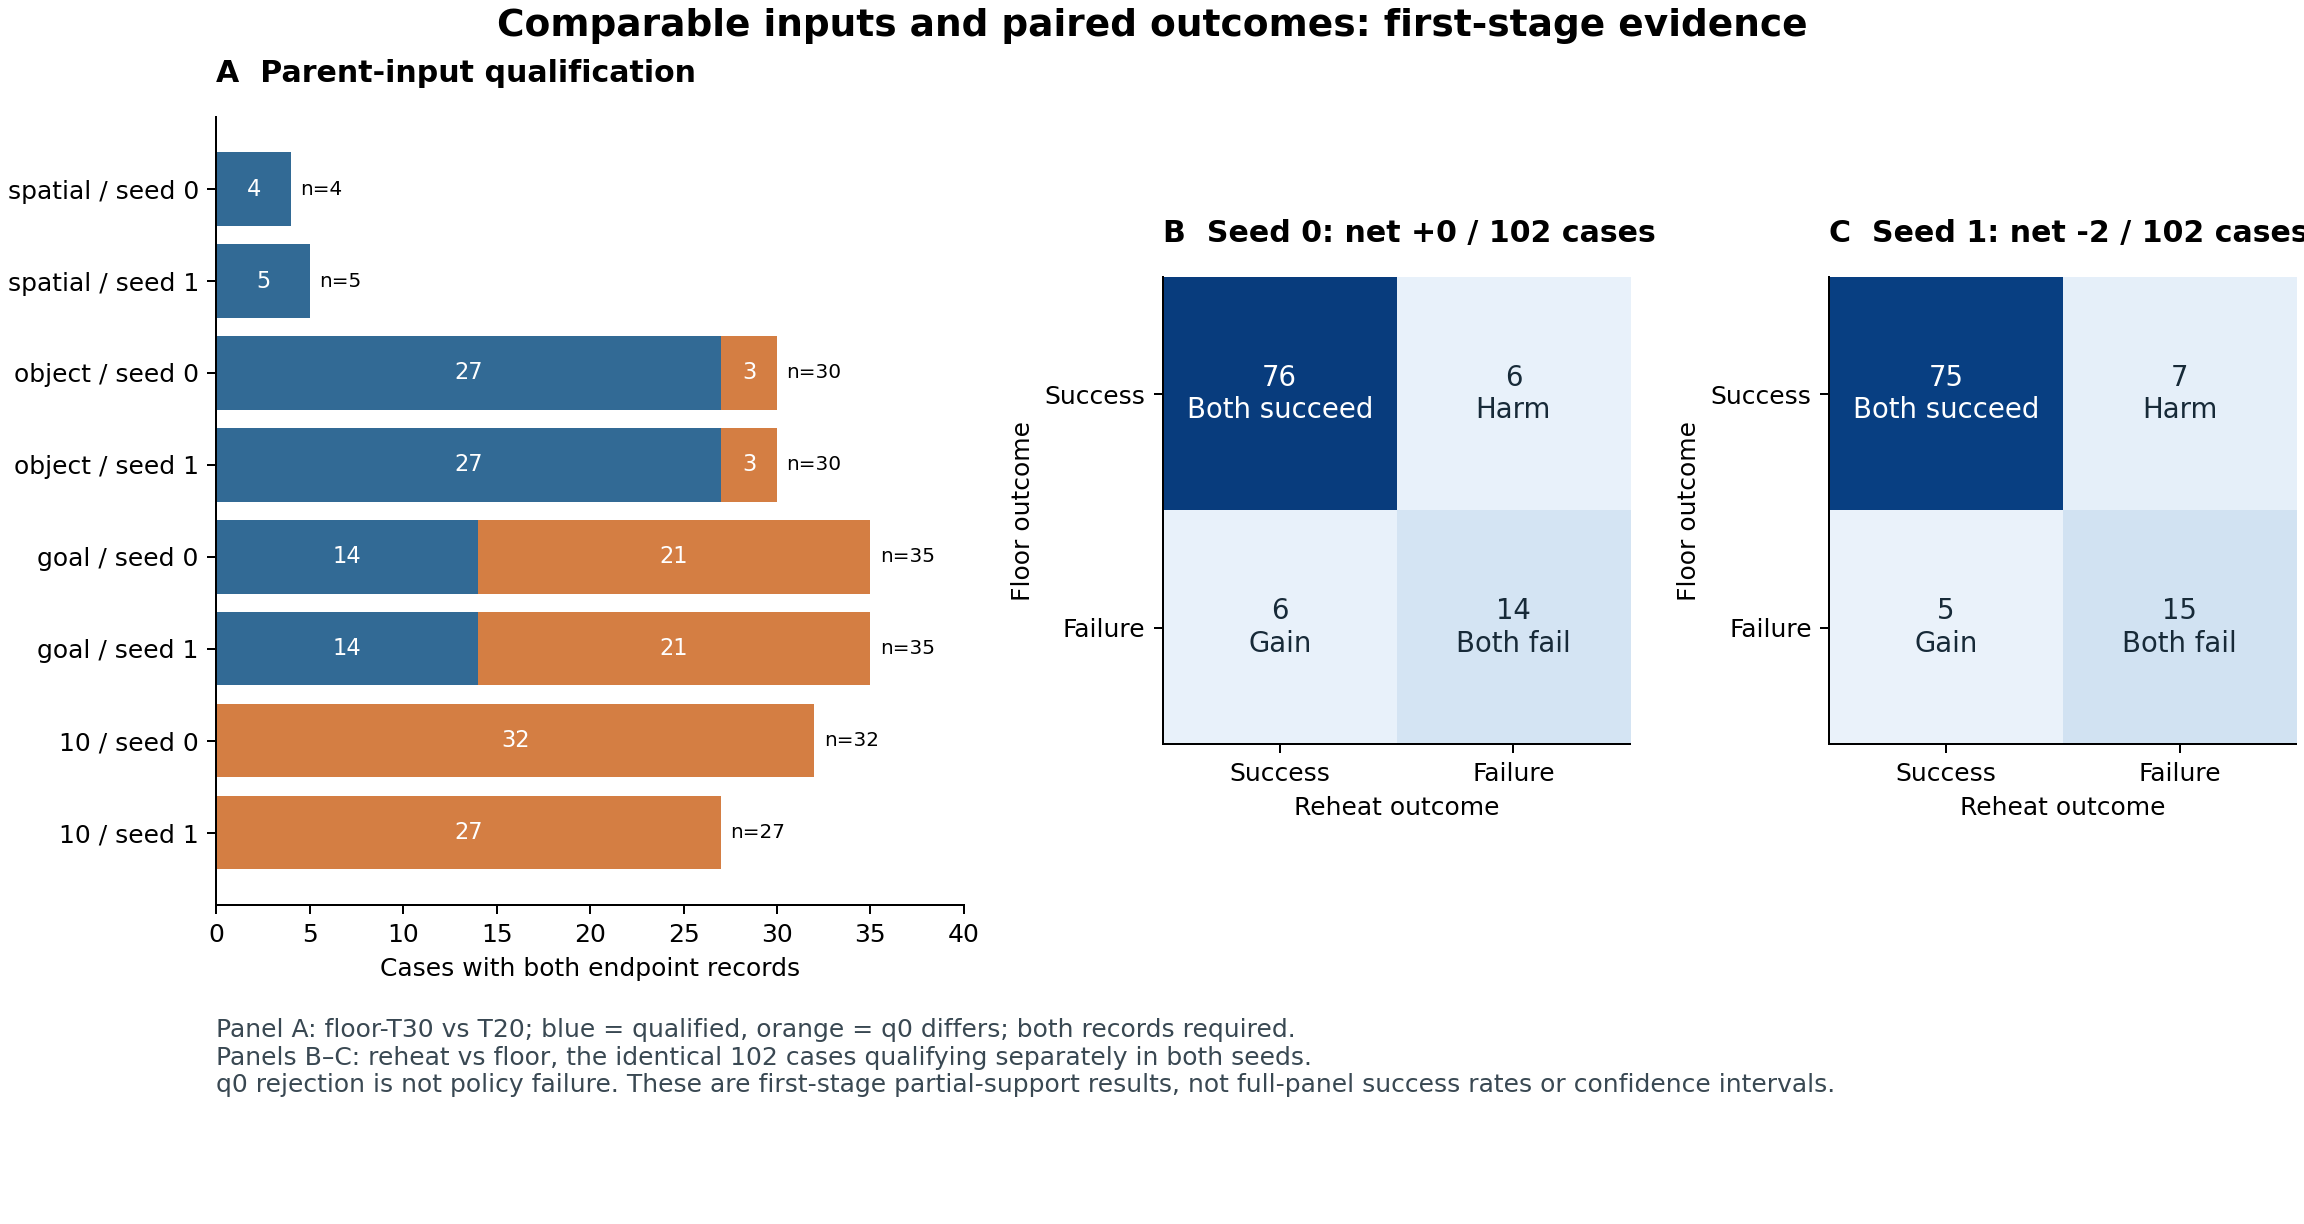
\includegraphics[width=\textwidth]{images/stage1-evidence.png}
\caption{First stratified-stage evidence. Left: floor-T30 versus its own T20 parent, showing only cases with both endpoint records. Input eligibility depends strongly on suite. Right: direct reheat versus floor on the identical 102 cases qualifying separately within each seed. Gains and harms largely cancel. These are partial-support results; rejected inputs are not policy failures.}
\label{fig:stage1}
\end{figure*}

\subsection{Parent comparisons expose structured input mismatch}
The new floor-to-parent comparisons contain 56/51 q0-rejected pairs for seeds 0/1; all 107 parent records come from the JD-derived evaluation cache. The remaining 45/46 eligible pairs come from the earlier BOS cache. This perfect source association within the sample does not identify a hardware cause.

A bounded CPU audit of all 107 rejected pairs reproduces the original rejection using complete archived fields. Physical-state payload hashes differ in all 107; end-effector position, quaternion, gripper position, main image and wrist image differ in 62, 26, 7, 52 and 56 pairs, respectively. Counts overlap. All 310 differing typed-array identities have matching dtype, shape, byte count and hash domain. Sixteen other fields, including the native initial state, initialization-file identity, scene, task specification, prompt, sensor RNG, inference noise and wait-step count, agree throughout. No field is missing. In 23 pairs only the physical-state hash differs.

Raw-input diagnostics on two fixed witnesses qualify this interpretation. Selected by the lowest seed/case identifier within two difference classes, their simulator-state maximum absolute differences are $5.55\!\times\!10^{-16}$ and $1.06\!\times\!10^{-15}$ in stored coordinates, not a uniform physical unit. The first has byte-identical images, proprioception and noise. The second has 1,339/65,536 main-camera and 455/65,536 wrist-camera pixels differing by at most one uint8 intensity level; proprioception and noise remain identical. Thus a hash mismatch need not imply a substantial visible-input change. These two diagnostics neither characterize all 107 pairs nor establish behavioral equivalence or a platform cause. The original exact gate remains unchanged. q0 precedes the first policy action: these differences are not feedback from that episode's learned actions. Simulator-state identity and model-visible input identity require separate interpretation.

\subsection{Coverage is not full-target identification}
Table~\ref{tab:coverage} counts adopted endpoints, including normal failures. Within the fixed Plus panel, all four T30 endpoints exist for 243 cases and all seven model endpoints for 230. Common T30 coverage reaches 39 of the 40 mapped task families, but the principal comparisons have both endpoints for only about 22--30\% of their predetermined mapped-task weight, before input rejection. Three thousand one hundred fifty-seven T30 panel endpoints and 229 parent/original reference endpoints remain missing. Missing execution, available results not yet joined into a particular analysis cache, and rejected pairs are tracked separately.

\begin{table}[t]
\caption{Adopted T30 endpoints at this revision. These cumulative historical counts are not matched-support success rates or a requirement to finish the original leaderboard.}
\label{tab:coverage}\centering
\begin{tabular}{@{}lrr@{}}
\toprule
Endpoint & Plus (success/failure) & Six-condition L10\\
\midrule
Floor s0 &2217 (1920/297)&34\\
Floor s1 &2120 (1803/317)&300\\
Reheat s0 &1116 (1029/87)&118\\
Reheat s1 &1617 (1467/150)&153\\
\midrule
Total &7070&605\\
\bottomrule
\end{tabular}
\end{table}

The full historical Original and T20 records provide additional system-level references, but their unequal initial inputs prohibit treating their score differences as isolated training effects. The custom L10 parents are especially sparse: only 22 of 300 cases per seed are closed; within the selected clean50 support only four per seed exist. More T30 evaluation does not itself resolve parent missingness or input mismatch.

\section{What Would Resolve the Question?}
The next step is to integrate already adopted endpoints into the fixed-panel cache, resolve the provenance and scale of input mismatches where archived data permit, and complete only genuine panel gaps that improve identification. A fixed case is not replaced because it fails or is ineligible. The analysis must show coverage and gains/harms for each seed, perturbation category, and base family. A result concentrated in one family changes the practical interpretation even if its aggregate sign is positive. Variant-level counts cannot be treated as independent task or training replicates; uncertainty analysis must respect this structure and cannot compensate for only two trained seeds.

Three outcomes would lead to different decisions. Broad, consistent gains over the parent, without compensating harms in the clean panel, would support additional optimization under the tested schedule. Consistent reheat benefits over floor would favor that future schedule as a whole. Persistent cancellation across well-covered families would motivate changing the training support or objective rather than simply adding updates. Current evidence cannot choose decisively between these outcomes.

A real-coordinate held-out readout, a stronger sampling baseline, or an independent setting could strengthen later claims, but they are not completed experiments and are not implied by the present results.

\section{Limitations and Conclusion}
The study currently covers one adapted model, two training seeds, one local demonstration split, and incomplete historical and stratified behavioral subsets. The original checkpoint's full upstream exposure history is not reconstructed, so local demonstration disjointness does not establish pretraining novelty. Two branches lack complete online logs and final held-out probe points. Technical eligibility may select atypical cases, and fixed recorded randomness does not guarantee all unrecorded intermediates are identical across runtimes. These limitations are part of the estimand, not defects that can be repaired by renaming a plot.

The evidence already separates three propositions: changing within-demonstration sampling changes held-out fitting; further optimization improves measured training-probe fitting; and its closed-loop benefit remains unresolved. Our next scientific decision is therefore to resolve the matched-support evidence for the existing intervention, rather than choose a branch by loss alone or launch a new mechanism story. A useful final result must tell a roboticist when further optimization is warranted, on what support, and with what behavioral tradeoff. The present manuscript supplies that testable structure and preliminary evidence; it does not claim that the final answer is already known.

\clearpage
\bibliographystyle{plainnat}
\begin{thebibliography}{8}
\bibitem{ross} S. Ross, G. J. Gordon, and J. A. Bagnell. A reduction of imitation learning and structured prediction to no-regret online learning. In \emph{AISTATS}, 2011.
\bibitem{pi05} Physical Intelligence et al. $\pi_{0.5}$: A vision-language-action model with open-world generalization. \emph{arXiv:2504.16054}, 2025.
\bibitem{oft} M. J. Kim, C. Finn, and P. Liang. Fine-tuning vision-language-action models: Optimizing speed and success. In \emph{Robotics: Science and Systems}, 2025.
\bibitem{scaling} F. Lin, Y. Hu, P. Sheng, C. Wen, J. You, and Y. Gao. Data scaling laws in imitation learning for robotic manipulation. \emph{arXiv:2410.18647}, 2024.
\bibitem{libero} B. Liu et al. LIBERO: Benchmarking knowledge transfer for lifelong robot learning. \emph{arXiv:2306.03310}, 2023.
\bibitem{plus} S. Fei et al. LIBERO-Plus: A progressive robustness benchmark for visual-language-action models. In \emph{CVPR}, 2026.
\bibitem{pro} X. Zhou et al. LIBERO-PRO: Towards robust and fair evaluation of vision-language-action models beyond memorization. \emph{arXiv:2510.03827}, 2025.
\bibitem{behavior} S. Higham, R. A. Izzo, M. Matteucci, and A. Suglia. Is success all you need? Investigating the impact of input perturbations on VLA behaviour in tabletop manipulation tasks. \emph{arXiv:2610.01351}, 2026.
\end{thebibliography}
\end{document}
